% Section content template for individual Educative lessons
% This file contains the actual content for a specific section
% Generated from Educative API section content

% Section: Getting Ready for the System Design Interview
% Section ID: 4771234193080320
% Section Slug: getting-ready-for-the-system-design-interview
% Generated: 2025-08-02T19:56:00.759893

A \textbf{System Design interview} is a technical evaluation of a candidate's ability to build robust and scalable systems. Unlike coding interviews, which typically involve a single solution, System Design interviews are open to discussion and involve multiple possible solutions that can be re-iterated.

For many software engineers, System Design Interview questions remain a mysterious challenge. Most engineers have never actually worked on large-scale systems before, so explaining how to build one seems daunting. Since System Design interview questions are often open-ended, it can be difficult to know the best way to prepare.

However, as someone who has participated in hundreds of System Design interviews, I can assure you there is a correct way to approach these questions. With the right mindset and preparation, you can feel confident and ready to tackle any System Design question that comes your way.

It is important to note that System Design questions not only test the technical knowledge of the candidate but also their ability to approach a problem, think critically, and make trade-offs. Therefore, preparing for a System Design interview is not only about understanding the technical details but also about understanding the problem, breaking it down, and finding the most optimal solution.

\begin{figure}[htbp]
 \centering
 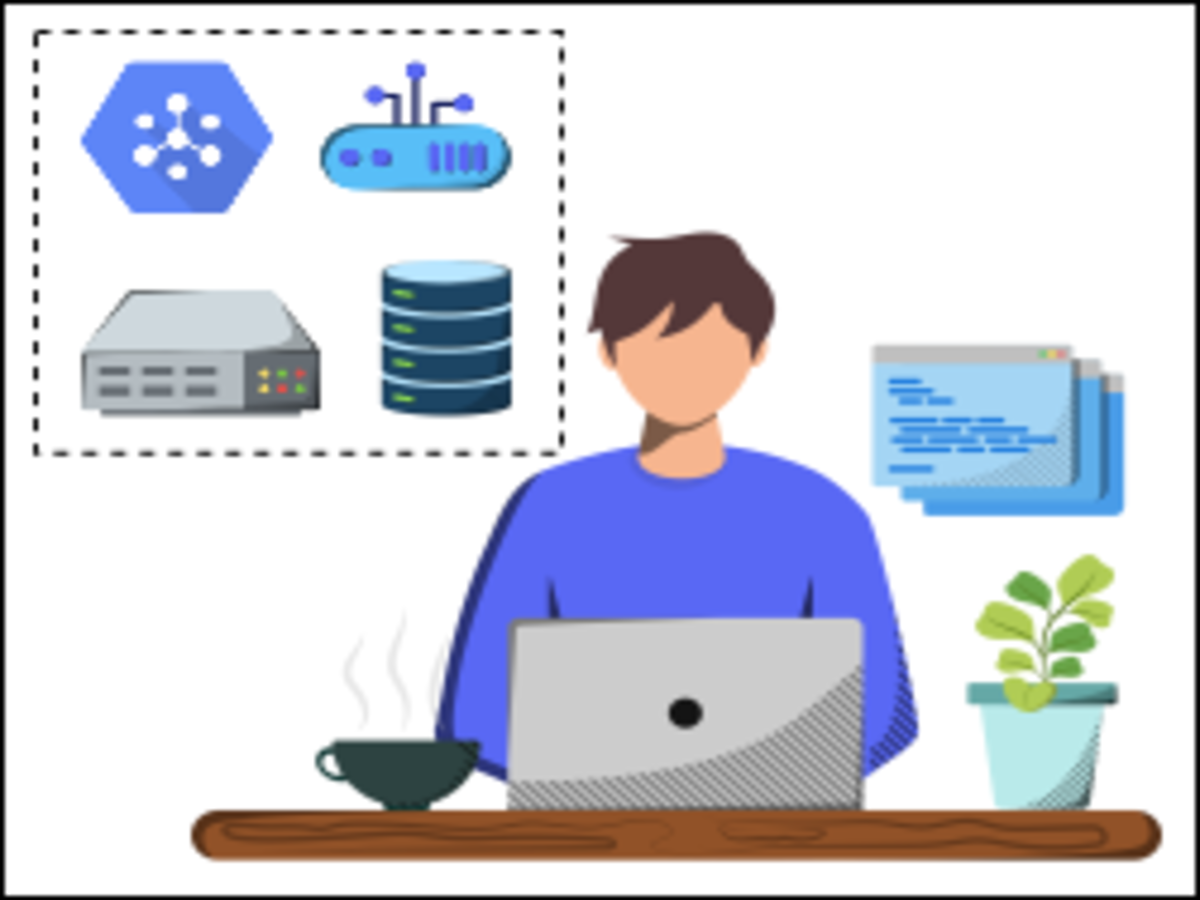
\includegraphics[width=0.8\textwidth]{Images/chapter_1/section_4771234193080320/4929411824877568.png}
 \caption{System Design interviews}
\end{figure}

\subsection{Author's background in System Design}\label{gIyZLoEnzqAWz9PwuDQ-5}

\noindent
\begin{minipage}[t]{0.48\textwidth}
Hi, I'm Fahim ul Haq, the co-founder of Educative and co-author of this course. In April 2008, I joined an \href{https://www.educative.io/blog/25-years-of-developer-interviews}{internal team at Microsoft} working on a large-scale project to build a distributed storage solution. Amazon launched its Simple Storage Service in 2006, and Google launched its PaaS solution, Google App Engine, the same month I joined the team, so we were in the early land grab of cloud computing. Less than two years later, that project was launched to the world as a new product category: Microsoft Azure.
\end{minipage}
\hfill
\begin{minipage}[t]{0.48\textwidth}

\includegraphics[width=0.8\textwidth]{Images/chapter_1/section_4771234193080320/4700286249992192.png}
\end{minipage}

When I joined the Azure team, I came from working on Exchange. I understood server storage and client management, but not at this scale and certainly not distributed across the world. It required a lot of learning on the job.

Today, the lessons I and other cloud engineers learned in those early days are codified into the System Design discipline. For many companies, the System Design Interview is instrumental in the developer interview process, which means it is vital for landing a job and setting your career on a good trajectory.

\subsubsection{What I learned through hundreds of System Design Interviews}\label{5Ai-AQby7BVCxBidhX3m3}

By the time I started Educative, I had participated in hundreds of interview loops as both interviewee and interviewer. As Educative has scaled, I have participated in hundreds more. The experience of working on web-scale systems at Facebook and Microsoft taught me two key skills for approaching the System Design Interview:

\begin{enumerate}
\item
\phantomsection\label{Ggzh5pTw39SD5OD34_J0H}
How to learn the fundamentals of distributed systems quickly and apply these principles in solving real-world problems
\item
\phantomsection\label{uaDMkBB3F04VJuTLg7hyL}
How to evaluate candidates while interviewing for System Design
\end{enumerate}

Here's the counterintuitive part: in the System Design Interview, companies are not actually trying to test your experience with System Design. Successful candidates rarely have much experience working on large-scale systems, and interviewers know this. Again , this discipline has only been around for about fifteen years, and like everything else in software engineering, it is evolving rapidly.
\begin{quote}
\textbf{Note:} The key is to prepare for the System Design interview with the intent to apply that knowledge.
\end{quote}
Our System Design course is equally useful for people already working and those preparing for interviews. In this chapter, we will highlight the different aspects of a System Design interview and some helpful tips for those who are preparing for an upcoming interview. We encourage learners to read this chapter even if they aren't preparing for an interview because some of the topics covered in this chapter can be applied broadly.

\subsection{How do System Design interviews differ from other interviews?}\label{NQeNxrqfHqs-dvlwL9oyU}

Just like with any other interview, we need to approach the System Design interviews strategically. System Design interviews are different from coding interviews. There's rarely any coding required in this interview.

\begin{figure}[htbp]
 \centering
 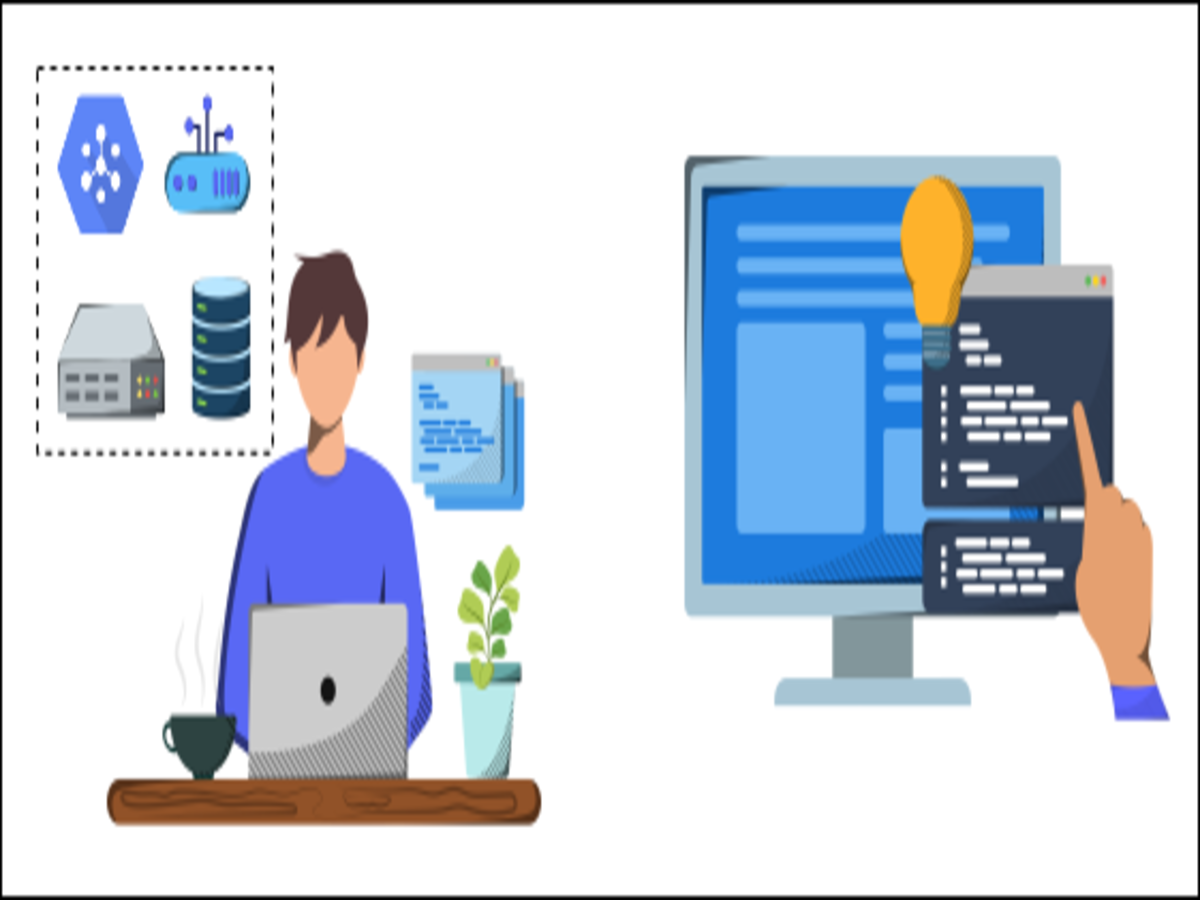
\includegraphics[width=0.8\textwidth]{Images/chapter_1/section_4771234193080320/5859851702239232.png}
 \caption{Other interviews versus a system design interviews}
\end{figure}

A System Design interview takes place at a much higher level of abstraction. We figure out the requirements and map them onto the computational components and the high-level communication protocols that connect these subsystems.

The final answer doesn't matter. What matters is the process and the journey that a good applicant takes the interviewer through.
\begin{quote}
\textbf{Note:}~As compared to coding problems in interviews, System Design is more aligned with the tasks we'll complete on our jobs.
\end{quote}
\subsection{How do we tackle a design question?}\label{V2_cowfLOR7_6lrU-55Oc}

Design questions are open ended, and they're intentionally vague to start with. Such vagueness mimics the reality of modern day business.

Interviewers often ask about a well-known problem---for example, designing WhatsApp. Now , a real WhatsApp application has numerous features, and including all of them as requirements for our WhatsApp clone might not be a wise idea due to the following reasons:

\begin{itemize}
\item
\phantomsection\label{0uEfb-y7Eteyhlt2HMQKn}
First, we'll have limited time during the interview.
\item
\phantomsection\label{TGDVjaDwtQ0YTnO7z7MNh}
Second, working with some core functionalities of the system should be enough to exhibit our problem-solving skills.
\end{itemize}

We can tell the interviewer that there are many other things that a real WhatsApp does that we don't intend to include in our design. If the interviewer has any objections, we can change our plan of action accordingly.

Here are some best practices that we should follow during a System Design interview:

\begin{figure}[htbp]
 \centering
 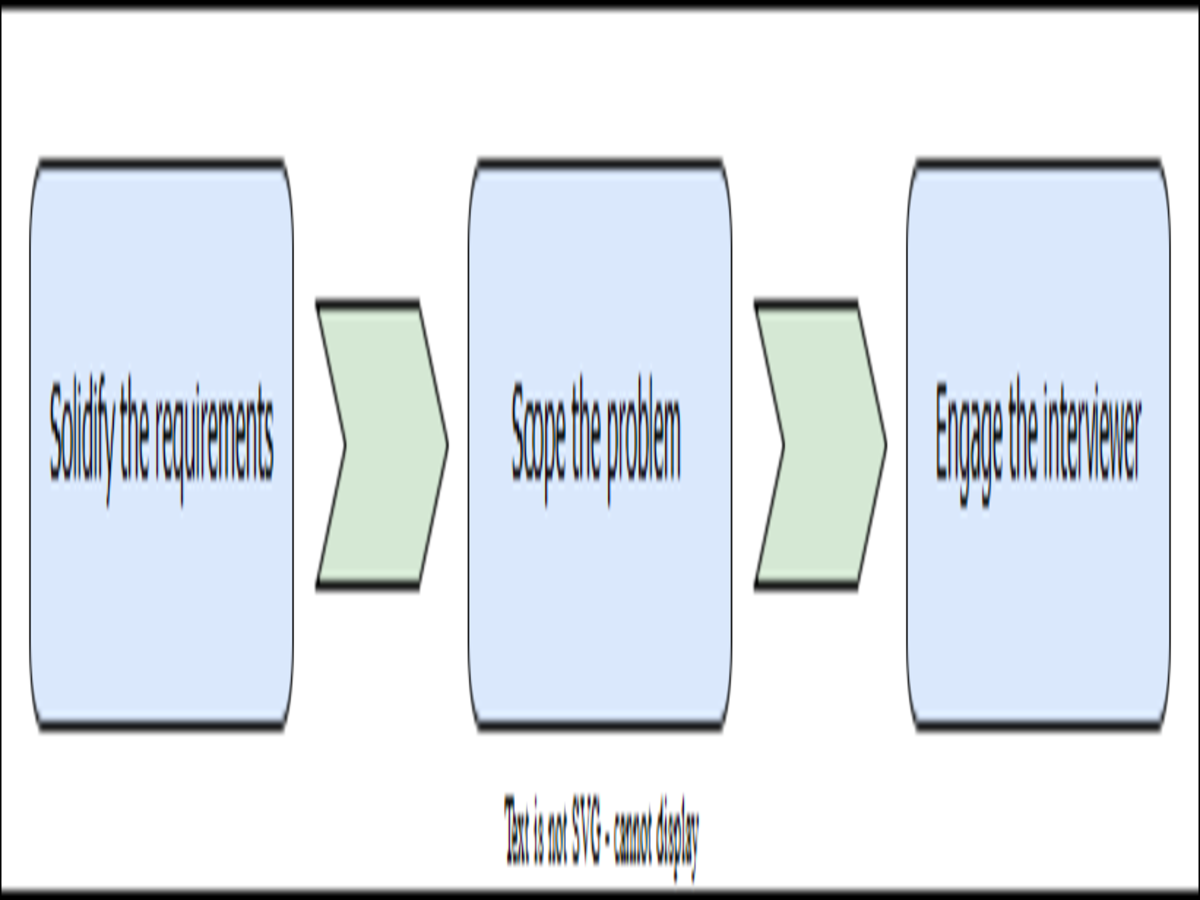
\includegraphics[width=0.8\textwidth]{Images/chapter_1/section_4771234193080320/4537563495137280.png}
 \caption{Best practices for the System Design interview}
\end{figure}

\begin{itemize}
\item
\phantomsection\label{BkHabk7AURmxR6IR-ch_a}
An applicant should ask the right questions to solidify the requirements.
\item
\phantomsection\label{tMnQnmcrx93uB5IFGVFMX}
Applicants also need to scope the problem so that they're able to make a good attempt at solving it within the limited time frame of the interview. System Design interviews are usually about 35 to 40 minutes long.
\item
\phantomsection\label{CncjPzeO-3fVJ2QM2o_ip}
Communication with the interviewer is critical. It's not a good idea to silently work on the design. Instead , we should engage with the interviewer to ensure that they understand our thought process.
\end{itemize}

\subsubsection{Present the high-level design}\label{RwSzNg6izH6FhCXOl7kS4}

At a high level, components could be frontend, load balancers, caches, data processing, and so on. The System Design explains how these components fit together.

An architectural design often represents components as boxes. The arrows between these boxes represent who talks to whom and how the boxes or components fit together collectively.

\begin{figure}[htbp]
 \centering
 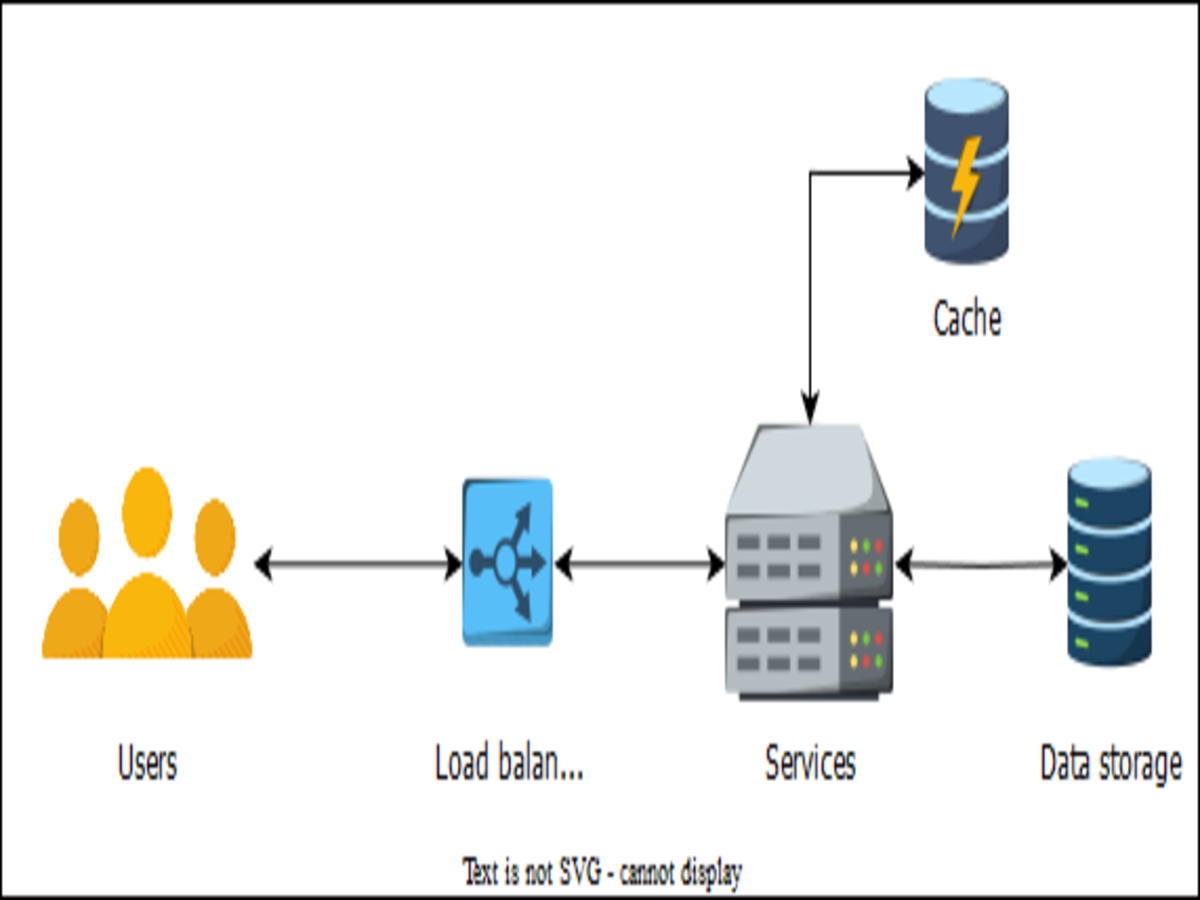
\includegraphics[width=0.8\textwidth]{Images/chapter_1/section_4771234193080320/6196252415229952.png}
 \caption{A sample design}
\end{figure}

\subsection{Possible questions for every System Design interview}\label{N0oqEUUvDaJbCsC9k12Oe}

System Design interviews often include questions related to how a design might evolve over time as some aspect of the system increases by some order of magnitude---for example, the number of users, the number of queries per second, and so on. It 's commonly believed in the systems community that when some aspect of the system increases by a factor of ten or more, the same design might not hold and might require change.

Designing and operating a bigger system requires careful thinking because designs often don't linearly scale with increasing demands on the system.

\begin{quote}
\textbf{Quiz:}
\textbf{Question 1:} Another question in a System Design interview might be related to why we don't design a system that's already capable of handling more work than necessary or predicted.
\textbf{Answer:} The cost associated with complex projects is a major reason why we don't do that.
\end{quote}

\subsubsection{Design challenges}\label{nZJnKsWiZ6bj_cIjKDdFU}

Things will change, and things will break over time because of the following:

\begin{itemize}
\item
\phantomsection\label{fiLYEOCeBPR1YLaGeiO7S}
There's no single correct approach or solution to a design problem.
\item
\phantomsection\label{IXq9Ed_IvPwtFnOuQuv7H}
A lot is predicated on the assumptions we make.
\end{itemize}

\subsubsection{The responsibility of the designer}\label{MTHYQVvlf7r6TLxOJsFHt}

As designers, we need to provide fault tolerance at the design level because almost all modern systems use off-the-shelf components, and there are millions of such components. So , something will always be breaking down, and we need to hide this undesirable reality from our customers.

\subsection{Who is eligible for a System Design interview?}\label{x5Sz5Sjx3GbmLnHTHXnIZ}

Traditionally, mid-to-senior level candidates with more than two years of experience get at least one System Design interview. For more senior applicants, two or three System Design interviews are common. Recently , large companies have also put forth System Design questions to some junior candidates. It
's never too early to learn System Design to grow or even expedite our careers.

\subsection{Theory and practice}\label{Theory-and-practice}

\noindent
\begin{minipage}[t]{0.48\textwidth}
Most of the theory of System Design comes from the domain of distributed systems. Getting a refresher on these concepts is highly recommended. Educative has an excellent~\href{https://www.educative.io/courses/distributed-systems-practitioners}{course on distributed systems}~that we can use to refresh our knowledge of distributed systems concepts.
\end{minipage}
\hfill
\begin{minipage}[t]{0.48\textwidth}

\includegraphics[width=0.8\textwidth]{Images/chapter_1/section_4771234193080320/5874390653075456.png}
\end{minipage}

Distributed systems give us guideposts for mature software principles. These include the following:

\begin{itemize}
\item
\phantomsection\label{8kWi4A5f2dvVaS_hyGAi2}
Robustness (the ability to maintain operations during a crisis)
\item
\phantomsection\label{n3X5NCP6M5Okm3RpeZFRy}
Scalability
\item
\phantomsection\label{wgHfXTx2euzdgaOwBdrv_}
Availability
\item
\phantomsection\label{Ao7XJxlae4646PY6EfSGQ}
Performance
\item
\phantomsection\label{UY-ZFRoBhpqHsi-D-u2X5}
Extensibility
\item
\phantomsection\label{2T30P2o-IzhDNLgBA_m8P}
Resiliency (the ability to return to normal operations over an acceptable period of time post-disruption)
\end{itemize}

Such terminology also acts as a lingua franca between the interviewer and the candidate.

As an example, we might say that we need to make a trade-off between availability and consistency when network components fail because the CAP theorem indicates that we can't have both under-network partitions. Such common language helps with communication and shows that we're well-versed in both theory and practice.

\subsubsection{When does the System Design interview occur in the hiring process?}\label{When-does-the-System-Design-interview-occur-in-the-hiring-process}

In FAANG+ (Facebook, Apple, Amazon, Netflix, Google, Microsoft, etc.), the hiring process involves several technical and non-technical interview rounds. The System Design interview usually comes after coding interview rounds and before behavioral interviews. A typical occurrence of a System Design interview in the hiring process is depicted below:

\begin{figure}[htbp]
 \centering
 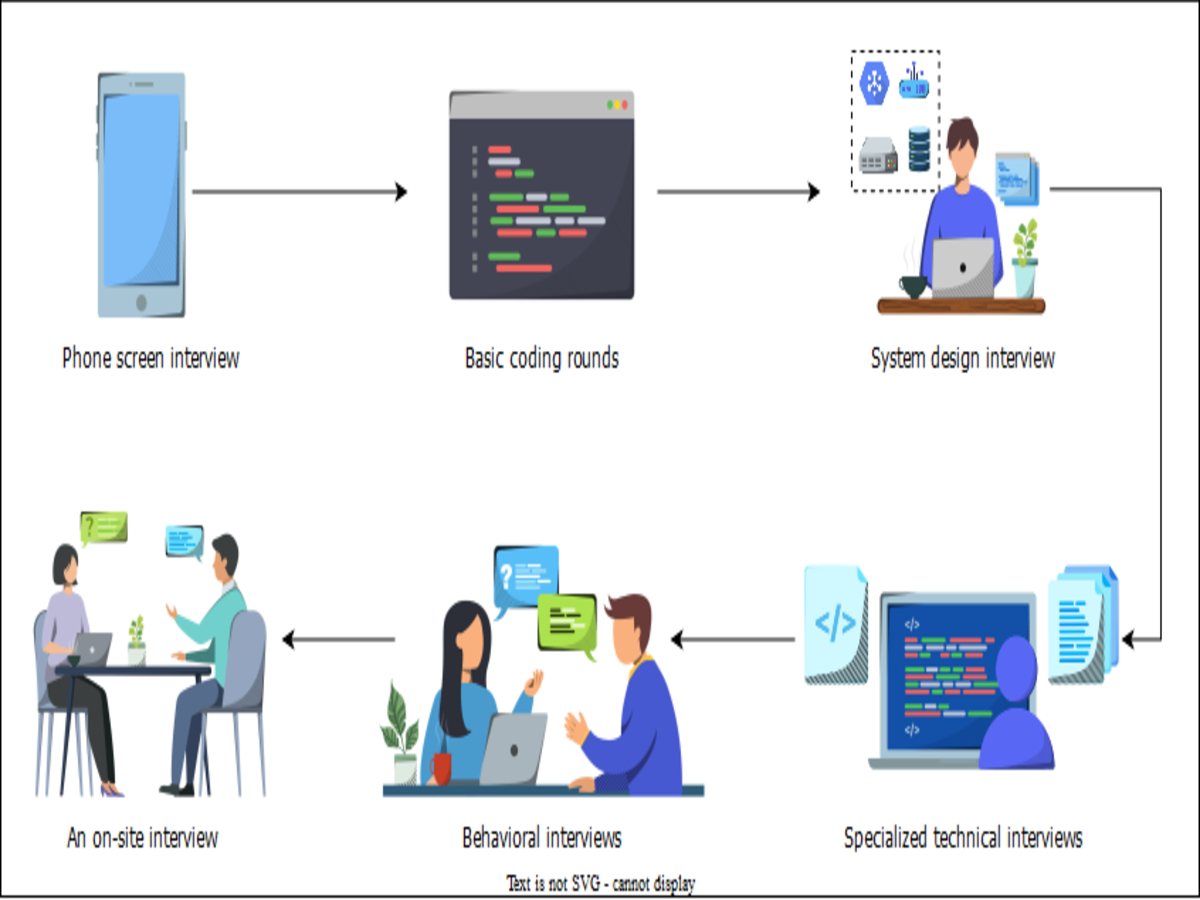
\includegraphics[width=0.8\textwidth]{Images/chapter_1/section_4771234193080320/6020586474438656.png}
 \caption{System Design interview, among other technical and nontechnical interviews}
\end{figure}

\begin{quote}
\textbf{Remember:}~In a System Design interview, It's a candidate's job to exhibit their skills to the interviewer.
\end{quote}

% End of section content